% -----------------------------------------------
% Template for SMC 2020
% adapted from previous SMC paper templates
% -----------------------------------------------

\documentclass[dvipsnames, pdftex]{article}
\usepackage{smc2020}
\usepackage{times}
\usepackage{ifpdf}
\usepackage[english]{babel}
\usepackage{cite}
\usepackage{amsmath}
\usepackage{textcomp}

\usepackage{xcolor}
\def\SWcomment[#1]{\textcolor{Red}{#1}}
\def\RPcomment[#1]{\textcolor{Blue}{#1}}
\def\SScomment[#1]{\textcolor{OliveGreen}{#1}}

%%%%%%%%%%%%%%%%%%%%%%%% Some useful packages %%%%%%%%%%%%%%%%%%%%%%%%%%%%%%%
%%%%%%%%%%%%%%%%%%%%%%%% See related documentation %%%%%%%%%%%%%%%%%%%%%%%%%%
%\usepackage{amsmath} % popular packages from Am. Math. Soc. Please use the 
%\usepackage{amssymb} % related math environments (split, subequation, cases,
%\usepackage{amsfonts}% multline, etc.)
%\usepackage{bm}      % Bold Math package, defines the command \bf{}
%\usepackage{paralist}% extended list environments
%%subfig.sty is the modern replacement for subfigure.sty. However, subfig.sty 
%%requires and automatically loads caption.sty which overrides class handling 
%%of captions. To prevent this problem, preload caption.sty with caption=false 
%\usepackage[caption=false]{caption}
%\usepackage[font=footnotesize]{subfig}


%user defined variables
\def\papertitle{Resurrecting the Tromba Marina: a bowed Virtual Reality instrument using haptic feedback and accurate physical modelling}

\def\firstauthor{Silvin Willemsen}
\def\secondauthor{Razvan Paisa}
\def\thirdauthor{Stefania Serafin}

% adds the automatic
% Saves a lot of output space in PDF... after conversion with the distiller
% Delete if you cannot get PS fonts working on your system.

% pdf-tex settings: detect automatically if run by latex or pdflatex
\newif\ifpdf
\ifx\pdfoutput\relax
\else
   \ifcase\pdfoutput
      \pdffalse
   \else
      \pdftrue
\fi

\ifpdf % compiling with pdflatex
  \usepackage[pdftex,
    pdftitle={\papertitle},
    pdfauthor={\firstauthor, \secondauthor, \thirdauthor},
    bookmarksnumbered, % use section numbers with bookmarks
    pdfstartview=XYZ % start with zoom=100% instead of full screen; 
                     % especially useful if working with a big screen :-)
   ]{hyperref}
  %\pdfcompresslevel=9

  \usepackage[pdftex]{graphicx}
  % declare the path(s) where your graphic files are and their extensions so 
  %you won't have to specify these with every instance of \includegraphics
  \graphicspath{{./figures/}}
  \DeclareGraphicsExtensions{.pdf,.jpeg,.png}

  \usepackage[figure,table]{hypcap}

\else % compiling with latex
  \usepackage[dvips,
    bookmarksnumbered, % use section numbers with bookmarks
    pdfstartview=XYZ % start with zoom=100% instead of full screen
  ]{hyperref}  % hyperrefs are active in the pdf file after conversion

  \usepackage[dvips]{epsfig,graphicx}
  % declare the path(s) where your graphic files are and their extensions so 
  %you won't have to specify these with every instance of \includegraphics
  \graphicspath{{./figures/}}
  \DeclareGraphicsExtensions{.eps}

  \usepackage[figure,table]{hypcap}
\fi

%setup the hyperref package - make the links black without a surrounding frame
\hypersetup{
    colorlinks,%
    citecolor=black,%
    filecolor=black,%
    linkcolor=black,%
    urlcolor=black
}


% Title.
% ------
\title{\papertitle}

% Authors
% Please note that submissions are NOT anonymous, therefore 
% authors' names have to be VISIBLE in your manuscript. 
%
% Single address
% To use with only one author or several with the same address
% ---------------
\oneauthor
   {\firstauthor, \secondauthor\ and \thirdauthor} {Multisensory Experience Lab, CREATE\\
  Aalborg University Copenhagen\\ %
    {\tt \href{mailto:sil@create.aau.dk}{\{sil, rpa, sts\}@create.aau.dk}}}

%Two addresses
%--------------
% \twoauthors
%   {\firstauthor} {Affiliation1 \\ %
%     {\tt \href{mailto:author1@smcnetwork.org}{author1@smcnetwork.org}}}
%   {\secondauthor} {Affiliation2 \\ %
%     {\tt \href{mailto:author2@smcnetwork.org}{author2@smcnetwork.org}}}

% Three addresses
% --------------
%  \threeauthors
%   {\firstauthor} {Affiliation1 \\ %
%      {\tt \href{mailto:author1@smcnetwork.org}{author1@smcnetwork.org}}}
%   {\secondauthor} {Affiliation2 \\ %
%      {\tt \href{mailto:author2@smcnetwork.org}{author2@smcnetwork.org}}}
%   {\thirdauthor} { Affiliation3 \\ %
%      {\tt \href{mailto:author3@smcnetwork.org}{author3@smcnetwork.org}}}


% ***************************************** the document starts here ***************
\begin{document}
%
\capstartfalse
\maketitle
\capstarttrue
%
\begin{abstract}
Tromba stuff Phantom omni

PHANTOM Omni for control and haptic feedback.

This paper presents the implementation and the evaluation of a VR bowed string instrument.  
Quick results

Commenting in colours :O \SWcomment[Silvin]{} \RPcomment[Razvan]{} \SScomment[Stefania]{}
\end{abstract}
%

\section{Introduction}\label{sec:introduction}
The tromba marina is a bowed monochord from medieval Europe \cite{encyclopaedia2020}. The string rests on a loose bridge that rattles against the body. This rattling mechanism creates a sound with brass- or trumpet-like qualities. Unlike other bowed string instruments, different frequencies are created by slightly damping the string with a finger of the non-bowing hand as opposed to pressing the string fully against the neck. This interaction at different locations along the string triggers the different harmonics of the open string. Furthermore, the tromba marina is bowed closer to the nut, and the finger determining the frequency is closer to the bridge (below the bow).

As the tromba marina is a rare instrument which can be merely found in museums, very few have the opportunity to play it.

In this paper, we aim to recreate a simulation of the feeling of playing this instrument by using physics based simulations and haptic feedback, together with a visual virtual reality experience.
Simulating the vibrations' feeling of a string instrument in particularly important since it has been shown how vibration's level can be strongly perceived \cite{askenfelt1992vibration}. 
%We want to emphasize that the visuals are only used for guiding the user, as we are most interested in the haptic feedback and audio.

Multisensory simulations for musical applications have shown some interest in the sound and music computing community. 
As stated in 
\cite{danieau2012enhancing}, the combination of haptics and audio visual content has its own specific challenges worth investigating.
Sile O'Modhrain is one of the pioneers that noticed the tight connection between auditory and haptic feedback and investigated how haptic feedback can improve the playability of virtual instruments \cite{o2001playing}.
At the same time, Charles Nichols developed the vBow, an haptic human computer interface for bowing \cite{nichols2002vbow}.
Researchers from ACROE in Grenoble have also developed for several years multisensory instruments based on the mass-spring-system paradigm, with custom-made bowing interfaces \cite{florens1990modeles,luciani2005action}.
Haptic feedback for digital waveguide models has also been investigated in \cite{sinclair2009audio}.

In this paper we aim to use democratized virtual reality technologies controlled by a commercial device called the
 PHANTOM Omni (or simply Omni) by SenseAble Technologies (now 3D Systems) \cite{phantom}.
 The PHANTOM Omni is a six-degrees-of-freedom system providing the haptic feedback in our application. Work using this controller in the context of audio include \cite{avanzini2006} and \cite{passalenti2019}, the latter of which is in the context of control of musical instruments, specifically on picking guitar strings.

Avanzini and Crosato test the influence of haptic and auditory cues on perception of material stiffness separately, but their work does not deal with musical instruments. Passalenti et. al's experiment focuses on guitar strings.
We start by describing the implementation of the system, both from the hardware and software perspective, and then we describe an experiment to evaluate..... 


\section{Hardware description}
The PHANTOM Omni (or simply Omni) is a six-degrees-of-freedom haptic system developed by SensAble Technologies. FireWire
\begin{figure}[ht]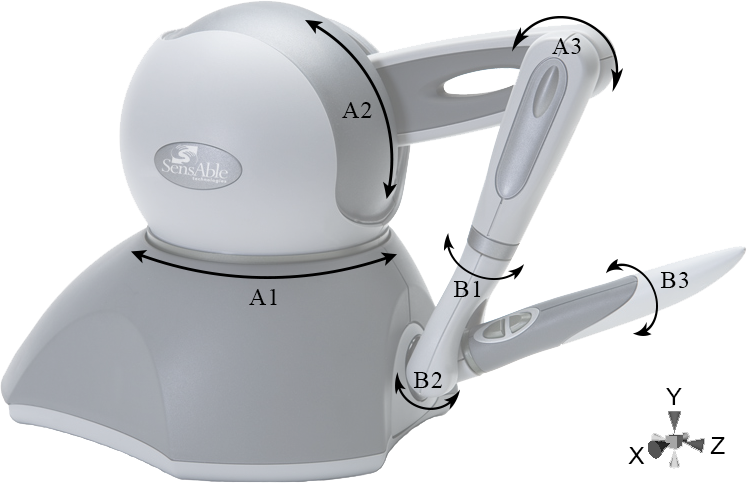
\includegraphics[width=1.0\columnwidth]{figures/omniSchematic.png}
\centering
  \caption{The PHANTOM Omni has six degrees of freedom, three of which provide force feedback (A1-3), and three only tracking position (B1-3). \label{fig:omni}}
\end{figure}

\section{Implementation}
The virtual tromba marina consists of several components: visuals, haptics and audio, all of which will be elaborated upon in this section. Then controls and mapping and finally the setup of the system will be presented.

\subsection{Visuals}
The application was built using cross-platform game engine Unity \cite{unity}. Unity can be used to build applications for Virtual Reality (VR) applications. A 3D model of the tromba marina was made inspired by a real-life instrument (presented in \cite{Baldwin2016}) available to the authors. Even though the visuals are not the focus of the implementation and eventual evaluation, it was used to guide the users movements and give them a sense of where the virtual instrument was located. Furthermore, a transparent white sphere was shown to indicate the location of the damping finger along the string. Moreover, some time was spent to make the scene `medieval' to match the instrument. \SWcomment[You could probably elaborate better here Razvan]

\subsection{Haptics}
The raw data provided by the Omni is the following:
\begin{itemize}
    \item absolute position of pivot point B2 (three degrees of freedom)
    \item rotation (three degrees of freedom)
    \item pressure (touching depth)
\end{itemize}
%
The axes are labelled as follows in relation to the virtual tromba marina: x-axis - width (horizontally across the soundboard -- the common interaction direction), y-axis - height (floor to ceiling) and z-axis - depth (horizontally perpendicular to the soundboard).


The end of the bow -- where a user normally holds it -- has been placed at the pivot point B2 \SWcomment[$\leftarrow$ is this true?]
The fact that pivot points B1-3 do not provide force feedback gives rise to an issue in our application. If the virtual
position of pivot point B2 is not the current point of interaction, in the extreme case when the user is bowing using the end of the bow, a force has to be applied as to not go through the string. To solve this issue, we created a separate object with which the bow (pivot point B2 to be exact) will interact with. The y-rotation and y-position of this exactly follows that of the Omni-pen and uses the virtual string as the centerpoint. The y-rotation will change the rotation of a local coordinate system (see Figure \ref{fig:localGlobal}. Furthermore, its (now local) x-position is determined by the distance between B2 and the string. 

\begin{figure}[ht]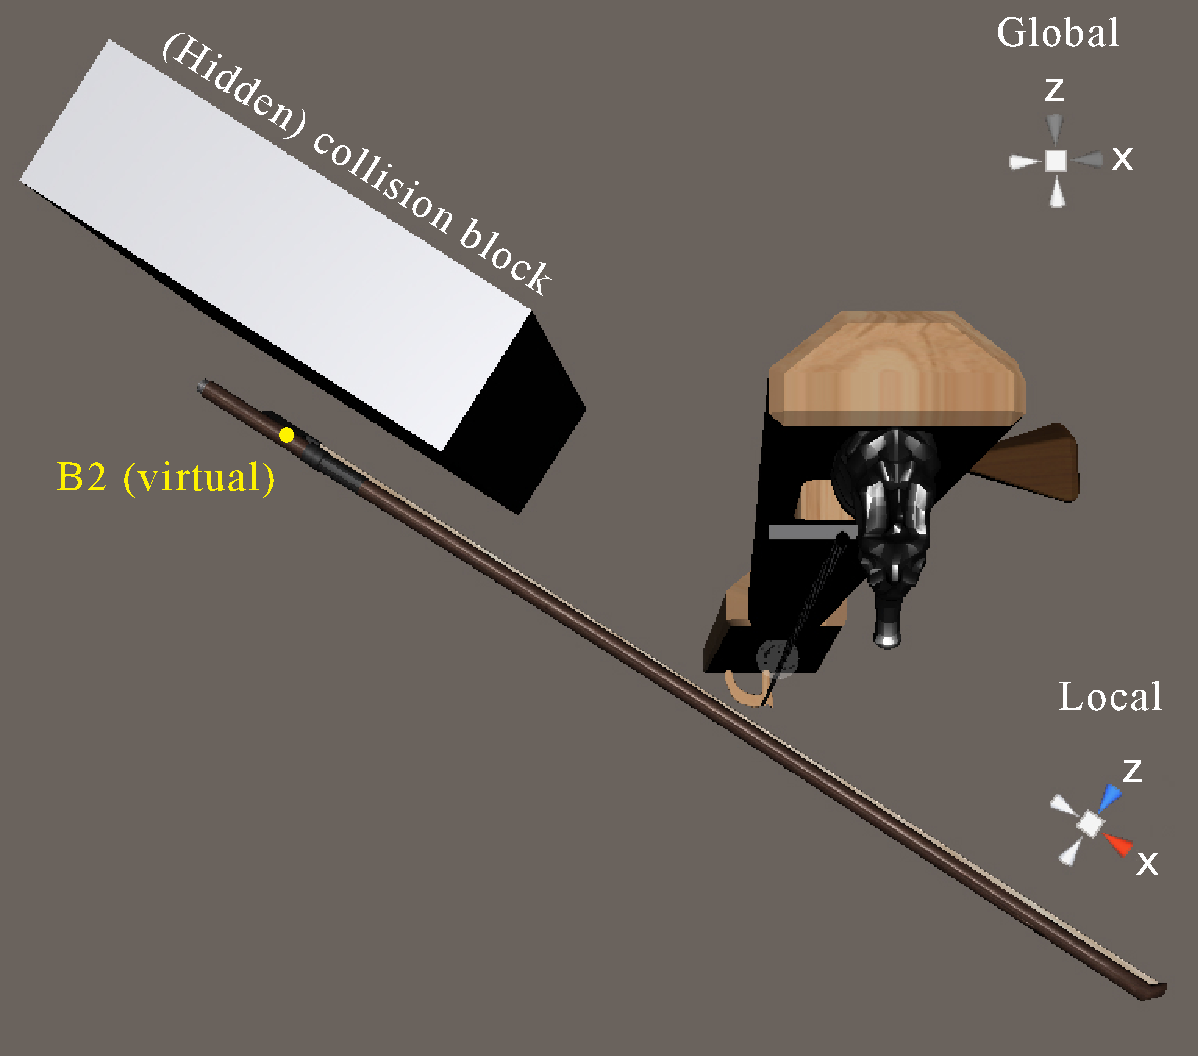
\includegraphics[width=1.0\columnwidth]{SMC 2020 paper template LaTeX/globalLocal.pdf}
\centering
  \caption{The local coordinate system with respect to the global coordinate system. Its rotation around the (global) y-axis is determined by the y-rotation of the bow. The (normally hidden) collision block lives in the local coordinate system. Its (local) x and y-position follows the (local) x and y-position of B2. \label{fig:localGlobal}}
\end{figure}

\subsection{Audio}
The audio is generated by a physical model of the tromba marina presented in a companion paper \cite{Willemsen2020}. The algorithm will not be discussed in detail here, but the mapping to the various parameters of the model will be described. 

Some parameters of the model are exposed to the Unity scene and can be controlled by the user. These are the velocity, force and position of the bow and the position of the finger inducing the harmonics.

\SWcomment[Talk about volume ratios? It's already discussed in the other paper]

\subsection{Controls and Mapping}\label{sec:controls}
As most people are right-handed, it was chosen to also have the bow in the right hand in the application. The (now-local) x-velocity of the Omni is mapped to the bow velocity, pressure to bow force and y-position to bow position. The left hand is used to control the pitch by changing the position of the damping finger along the string. This position is defined as  
\begin{equation}\label{eq:node}
    x_\text{f} = L\cdot n^{-1},
\end{equation}
where $L$ is the length of the string and $n \in [2,8]$. If $n$ is an integer, it is the number of the harmonic we want to induce. The lowest harmonic has been set at half the string length $L/2$, meaning that the string is never completely open. The highest harmonic (8 in this case) has been chosen to be the one that can still be (comfortably) played. The location of the damping finger $x_\text{f}$ is controlled using the `X' and `Y' buttons and the joystick on the left Oculus controller (see Figure \ref{fig:oculusController}). The buttons are for ``discrete harmonic" control of the damping finger, i.e. integer values of $n$ in Equation \eqref{eq:node}, where `Y' increases $n$ and `X' decreases it. The joystick allows for fine pitch control, i.e., decimal values of $n$,  and moves the damping finger up and down the string. The latter could potentially create pitch glides in the output sound of the application, but make it harder to `hit' a perfect harmonic according to Equation \eqref{eq:node}. If a button is pressed while the current finger position is between two discrete points, the position will move to the next or previous discrete position, depending on the button pressed.
%As the position of the first node along the string is at \begin{equation}\label{eq:node}
%     x_\text{node} = L\cdot n^{-1},
% \end{equation}
% where $L$ is the length of the string and $n \in [2,8]$ is the harmonic number, we want the damping finger to be set to these positions to induce these harmonics. The lowest harmonic has been set at half the string length $L/2$, meaning that the string is never completely open. The highest harmonic has been chosen to be the one that can still be (comfortably) played. The location of the damping finger ($x_\text{f}$) is controlled using the `X' and `Y' buttons and the joystick on the left Oculus controller (see Figure \ref{fig:oculusController}). The buttons are for discrete control of the damping finger, where `Y' increases $n$ in Equation \eqref{eq:node} and `X' decreases it. The joystick allows for fine pitch control  and moves the damping finger up and down the string. The latter could potentially create pitch glides in the output sound of the application, but make it harder to `hit' a perfect harmonic according to Equation \eqref{eq:node}. If a button is pressed while the current finger position is between two discrete points, the position will move to the next or previous discrete position, depending on the button pressed.

\begin{figure}[ht]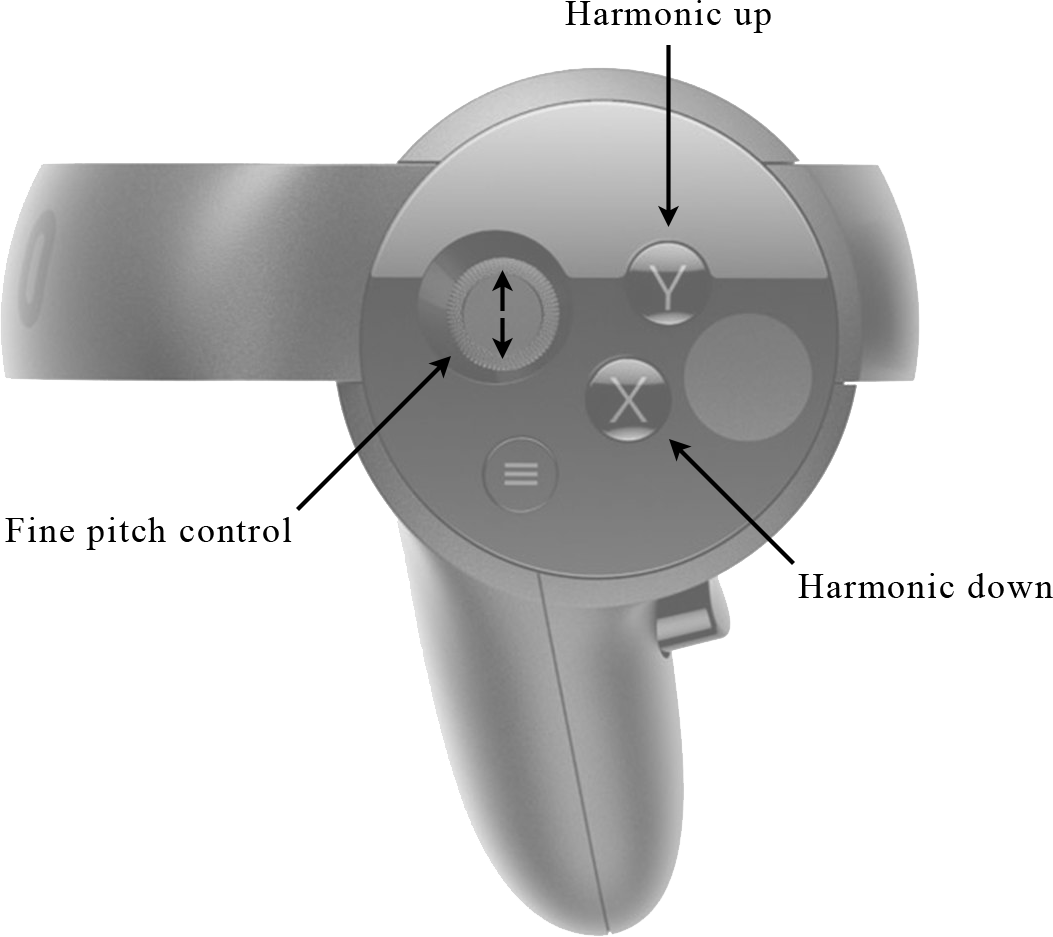
\includegraphics[width=1.0\columnwidth]{SMC 2020 paper template LaTeX/figures/controller.png}
\centering
  \caption{The left Oculus Touch controller. The controls for changing the pitch are highlighted. \label{fig:oculusController}}
\end{figure}
\subsection{Physical setup}\label{subsec:physicalSetup}
The physical setup is shown in Figure \ref{fig:physicalSetup}

The Omni is mounted on a stand at \texttildelow125 cm to match the approximate bowing height of the real instrument. As can be seen in Figure \ref{fig:physicalSetup}, the right Oculus Touch controller is mounted right underneath the Omni. This is used to align the physical setup with the virtual tromba marina, both in the x-z--plane but also the height of the bow in the application. After the scene is initialised the controller is used for a tilting interaction so that the instrument can rest on the user's shoulder. 

(something about the right Oculus Touch controller determining position and alignment )

A diagram showing the setup of the system can be found in Figure \ref{fig:systemLayout}. The user controls the application using the Omni and the left Oculus Touch controller which sends data to the PC running the application. The Omni sends haptic data back depending on the position and rotation data of pivot point B2. This data triggers the physical model which sends sound to a pair of speakers. The user wears a head-mounted display (HMD) that gives visual information about the location of the tromba marina (and medieval setting) \SWcomment[Different wording or elaboration]. The user's position in the VR environment is controlled by the HMD but this dataflow is not visualised in the diagram. Lastly, the right Oculus Touch controller is attached to the 

\begin{figure}[ht]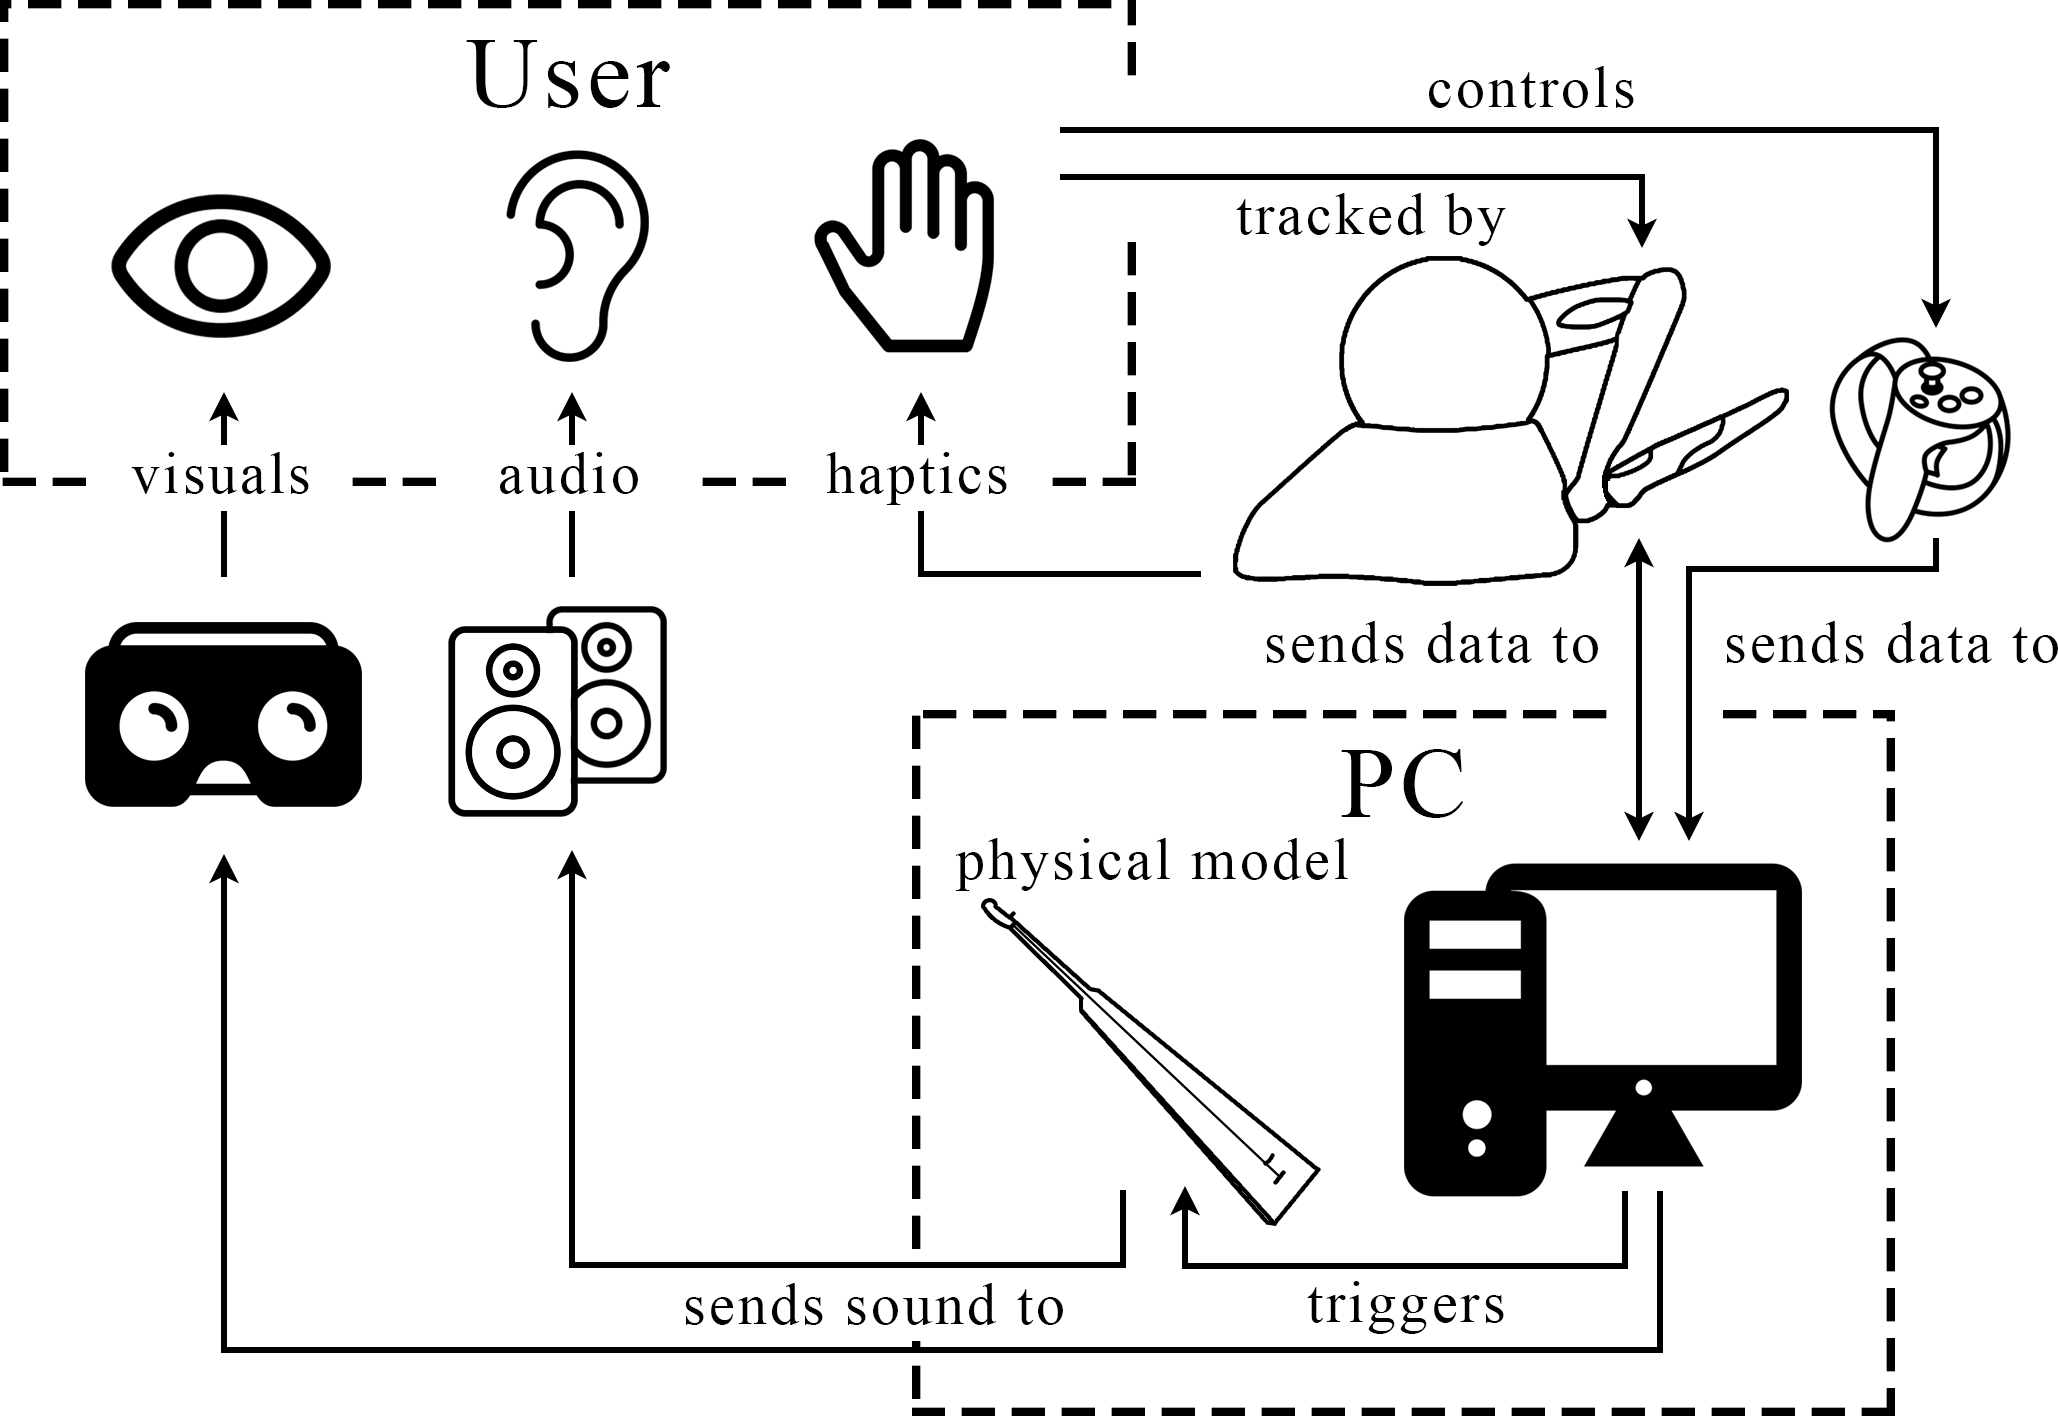
\includegraphics[width=1.0\columnwidth]{SMC 2020 paper template LaTeX/figures/blockdiagram.png}
\centering
  \caption{Diagram showing the system layout of the application. The user interacts with the system using the Omni -- which in turn provides haptic feedback -- and the Oculus Touch controller. These trigger the physical model of the tromba marina. Auditory feedback then comes from speakers and visual feedback from the Oculus Rift headset. A detailed explanation can be found in Section \ref{subsec:physicalSetup}. \label{fig:systemLayout}}
\end{figure}

\section{Evaluation}
The evaluation was inspired by \cite{Young2003} \cite{Someren1994} \cite{Stowell2009} and \cite{Finstad2010} \SWcomment[(obviously this will be elaborated upon)]

The goal of the evaluation was not to test minute interactions, but rather the general experience and the playability of our application. In total, 14 people participated in our experiment, all of which had at least one year of experience playing an instrument. This section will run through the setup of the experiment and the methods we used.

The experiment started with the participant reading an introduction about the experiment and answering several demographic questions. Then the application and controls were presented after which the participant started the experiment. It was emphasised that the most important part of the experiment was for the participant to speak their mind, ``anything positive, negative, basically anything that comes to mind, please speak out loud". Furthermore, the user was instructed to bow above the damping finger (visualised as a white sphere) at all times, as this is also the interaction with the real instrument. 

The interaction part was divided into two phases. Firstly, the participants are asked to explore the instrument on their own. Then, when they felt they are ready to move on, an audio clip made by the authors using the application was played to show what was possible with the application to inspire the second round of free exploration. It was stressed that the participants did not have to recreate what they heard, but to merely use it as inspiration. Their actions were observed throughout both phases and noted down as well as their speech. When they felt like they were ready to stop, they were asked to fill out a range of questions about their experience. Their answers were recorded on a 5-point Likert scale (strongly disagree - strongly agree). Finally, a semi-structured interview was held which lasted 5 minutes on average. The full experiment lasted \texttildelow30 minutes for all participants.

\section{Results}
In this section, both the quantitative and qualitative results will be given (and discussed) \SWcomment[Separate section for results and discussion I suppose]
\subsection{Quantitative data}
\subsection{Qualitative data}
Many users noted that the full range of the bow could not be used

Some noted that the control of the damping finger (`Y' for up the string and `X' for down, likewise for the joystick) should have been inversed. Furthermore, some would have liked a more physical interaction for the damping finger, such as moving the controller up and down rather than using buttons. This makes sense... \SWcomment[more here]

Interestingly, many participants believed that it was easy to play the instrument, but that they could become better after some more practice. This shows that the setup has a gentle learning curve, with an envisioned high virtuosity level \SWcomment[one does not imply the other directly (so might want to use different wording here) but it would be good to touch upon this]

Many noticed that the bow could rotate along its axis and asked whether it made a difference to which we always answered negatively. 

Some participants noted that they wanted to recreate the example sound, but couldn't because it sounded way more distorted. We recorded the example where the plugin was set to maximum volume causing clipping to the sound. The volume was turned down during the test to make it less distorted, but the recording was not remade.
% \begin{figure}[ht]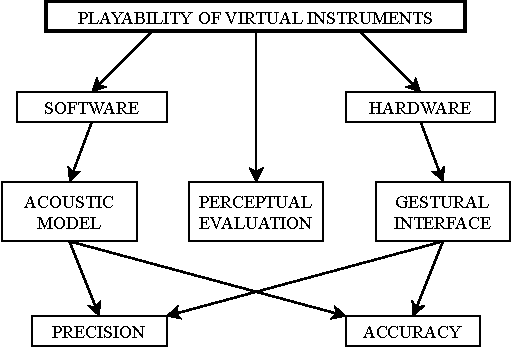
\includegraphics[width=1.0\columnwidth]{SMC 2020 paper template LaTeX/figures/PlayabilityChart.pdf}
% \centering
%   \caption{Playability chart of a virtual musical instrument \cite{Young2003}. \label{fig:oculusController}}
% \end{figure}

\section{Discussion}\label{sec:discussion}
Cognitive load of speech and playing an instrument are ``the same" (Paisa, 2020). So participants speaking their mind while playing might be an issue. Most probably, they will alter between playing and ``thinking aloud". 

\section{Conclusions}
test

\begin{acknowledgments}
We would like to thank all participants for taking the time to test our implementation...
\end{acknowledgments} 

%%%%%%%%%%%%%%%%%%%%%%%%%%%%%%%%%%%%%%%%%%%%%%%%%%%%%%%%%%%%%%%%%%%%%%%%%%%%%
%bibliography here
\bibliography{smc2020bib}

\end{document}
